\documentclass[11pt]{article}
\usepackage[utf8]{inputenc}
\usepackage[shortlabels]{enumitem}
\usepackage{cite}
\usepackage{graphicx}
\usepackage{amsmath}
\usepackage{esint}
\usepackage{units}
\usepackage{siunitx}
\usepackage{parskip}
\usepackage{mdframed}
\usepackage{amssymb}
\usepackage{commath}
\usepackage{subfig}
\usepackage{float}
\usepackage[hidelinks]{hyperref}
\usepackage[top=2.54cm, bottom=2.54cm]{geometry}

\sisetup{
	per-mode=fraction,
	fraction-function=\tfrac
}

\title{Smoothness\\
    \large Multivariable Calculus}
\author{Martin Gong / Nanami Kyosuke}

\begin{document}
    \maketitle

    \section{Intuitive Sense}

    \hfil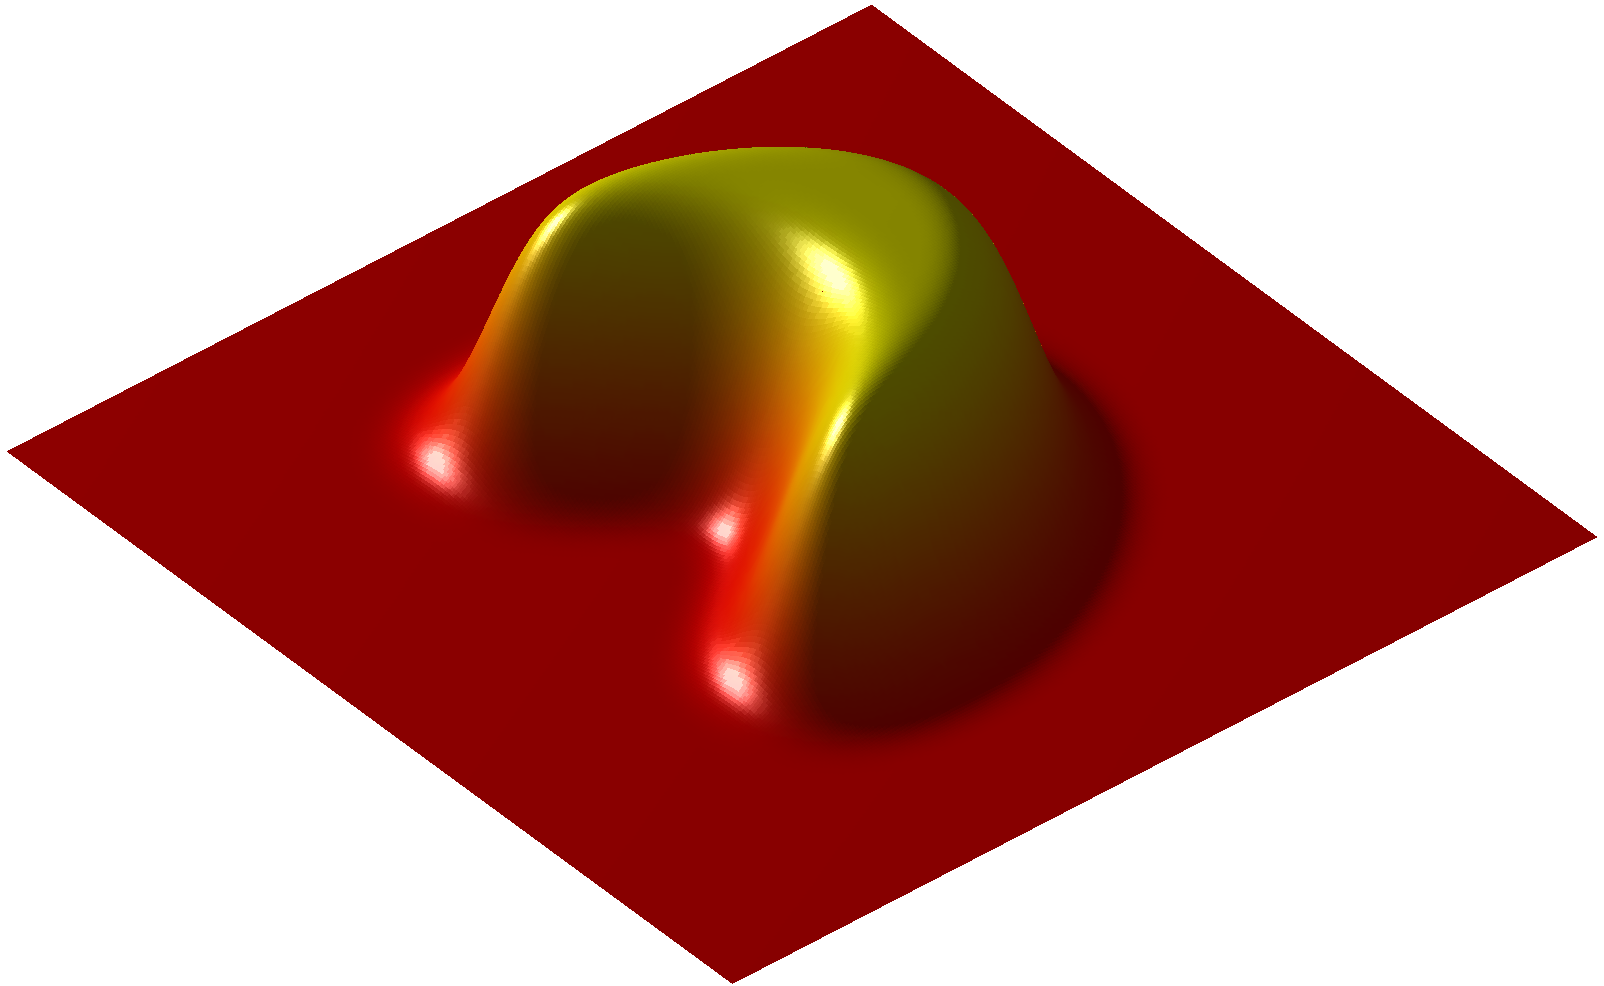
\includegraphics[scale=0.5]{assets/smoothness-1.png}

    For a curve to be considered smooth, it needs to be \textit{smooth}. There cannot be corners.

    \section{Mathematical Sense}

    To express that some function $f(x)$ is smooth, we express it with the differentiability class

    \[f(x) \in C^{(n)} \vert n \in \mathbb{N}\]

    In other words, all derivative functions of $f(x)$, up to the $n^{th}$ derivative of the function, are continuous.

    If a functions is in itself continuous, then

    \[f(x) \in C^{(0)}\]

    This is also the minimum requirement for a ``smooth'' curve.

    A curve can also be differentiable for derivative of all orders in its domain, where it is called ``infinity differentiable''

    \[f(x) \in C^{(\infty)}\]

    \section{Examples}

    \begin{enumerate}
        \item $f(x) = 0$ is considered smooth, and also infinitely differentiable, since derivatives of any order is 0.
    
        \item $e^x$ is also smooth and infinitely differentiable, since it stays the same.
    
        \item $\sin(x)$ is also a function that is differentiable for all orders.
    \end{enumerate}

\end{document}